\documentclass[12pt]{article}
\setlength\parindent{0pt}
\usepackage{amsmath}
\usepackage{lscape}
\usepackage{graphicx}
\usepackage{fullpage}
\usepackage[margin=0.8in]{geometry}
\setlength{\parskip}{4mm}
\def\LL{\left\langle}   % left angle bracket
\def\RR{\right\rangle}  % right angle bracket
\def\LP{\left(}         % left parenthesis
\def\RP{\right)}        % right parenthesis
\def\LB{\left\{}        % left curly bracket
\def\RB{\right\}}       % right curly bracket
\def\PAR#1#2{ {{\partial #1}\over{\partial #2}} }
\def\PARTWO#1#2{ {{\partial^2 #1}\over{\partial #2}^2} }
\def\PARTWOMIX#1#2#3{ {{\partial^2 #1}\over{\partial #2 \partial #3}} }
\newcommand{\BE}{\begin{displaymath}}
\newcommand{\EE}{\end{displaymath}}
\newcommand{\BNE}{\begin{equation}}
\newcommand{\ENE}{\end{equation}}
\newcommand{\BEA}{\begin{eqnarray}}
\newcommand{\EEA}{\nonumber\end{eqnarray}}
\newcommand{\EL}{\nonumber\\}
\newcommand{\la}[1]{\label{#1}}
\newcommand{\ie}{{\em i.e.\ }}
\newcommand{\eg}{{\em e.\,g.\ }}
\newcommand{\cf}{cf.\ }
\newcommand{\etc}{etc.\ }
\newcommand{\Tr}{{\rm tr}}
\newcommand{\etal}{{\it et al.}}
\newcommand{\OL}[1]{\overline{#1}\ } % overline
\newcommand{\OLL}[1]{\overline{\overline{#1}}\ } % double overline
\newcommand{\OON}{\frac{1}{N}} % "one over N"
\newcommand{\OOX}[1]{\frac{1}{#1}} % "one over X"
\pagenumbering{gobble}
\begin{document}
\Large
\centerline{\sc{Homework -- Light and Thermal Radiation}}

\normalsize
\begin{center}
	Due Thursday, October 28, before the beginning of class
\end{center}

\bigskip

\section{Reference for the Electromagnetic Spectrum}

The relationships between wavelength, frequency, and photon energy, as well as the names of different ``colors'' of light, are shown on this chart from Lawrence Berkeley National Laboratory:

\begin{minipage}{0.35\textwidth}
	Note here that the wavelength, frequency, and photon energy are shown in scientific notation. As the wavelength gets shorter, both the frequency and the energy of one photon increase.
	\end{minipage}
\hspace{0.05\textwidth}
\begin{minipage}{0.\textwidth}
\begin{center}
	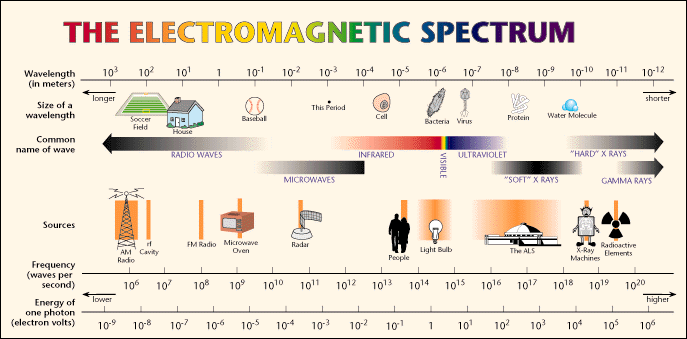
\includegraphics[width=4in]{EMSpec.png}
\end{center}
	\end{minipage}


The visible range is roughly from 380 nm (blue) to 750 nm (red).6

\section{Reference for Thermal Radiation}

(If you are looking at this before Tuesday's class and it doesn't make sense -- don't worry! We'll talk about this then.)

There is also a relationship between the temperature of an object and the type of light it emits. As the temperature of an object increases:

\begin{itemize}
	\item The types of light it emits shift to shorter wavelengths
	\item It emits much {\it more} light
\end{itemize}

This is a range, however: an object that {\it mostly} emits visible light, like the Sun, will also emit some near infrared and ultraviolet, too.

Everything on the chart is approximate. 

\begin{tabular}{|c|c|c|}
	\hline
	\bf Example & \bf Temperature (Kelvin) & \bf Peak Emission \\ \hline
	Deep space & 3 K & Microwaves \\ \hline
	Room temperature & 300 K & Far infrared \\ \hline
	A hot stove & 1000 K & Near infrared (plus a little bit of visible) \\ \hline
	A ``cool'' star & 3500 K & Red (plus a lot of infrared)\\ \hline
	The Sun & 5800 K & Visible light (even balance) \\ \hline
	A ``hot'' star & 10,000 K & Blue (plus a lot of ultraviolet) \\ \hline
	The hottest stars & 100,000 K & Ultraviolet \\ \hline
	Gas falling into a black hole & 1 million K & X-rays \\ \hline
\end{tabular}


\section{Questions for Homework}

\begin{enumerate}
	\item Photons with more than about 10 eV of energy per photon are capable of ionizing atoms -- tearing their electrons off. If this happens to atoms that are part of your body, this can cause chemical change that can make you sick or cause genetic changes that can lead to cancer.
	
	What types of light are capable of doing this?
	
	\item Wifi uses either 2.4 GHz or 5 GHz to carry its signals. Which one has longer wavelength?
	
	\item Photons that comprise visible light range from 1.6 eV to 3.2 eV (approximately). What color are 1.6 eV photons? What color are 3.2 eV photons? (Note that blue and violet have short wavelengths, and red has long wavelengths.)
	
	\item We often think of red as a `warm" color and blue as a ``cool'' color. Is this correct? If you see a blue star and a red star, which one is hotter?
	
	\item You observe two stars that produce the spectral curves shown here.
	
	\begin{minipage}{0.5\textwidth}If they are the same distance away, explain:
		
	\begin{enumerate}
	\item Which star would look brighter?
	\item What color would each star appear to be to the eye?
	\item Which star is larger?
	\end{enumerate}
	\end{minipage}
\hspace{0.05\textwidth}
	\begin{minipage}{0.4\textwidth}
	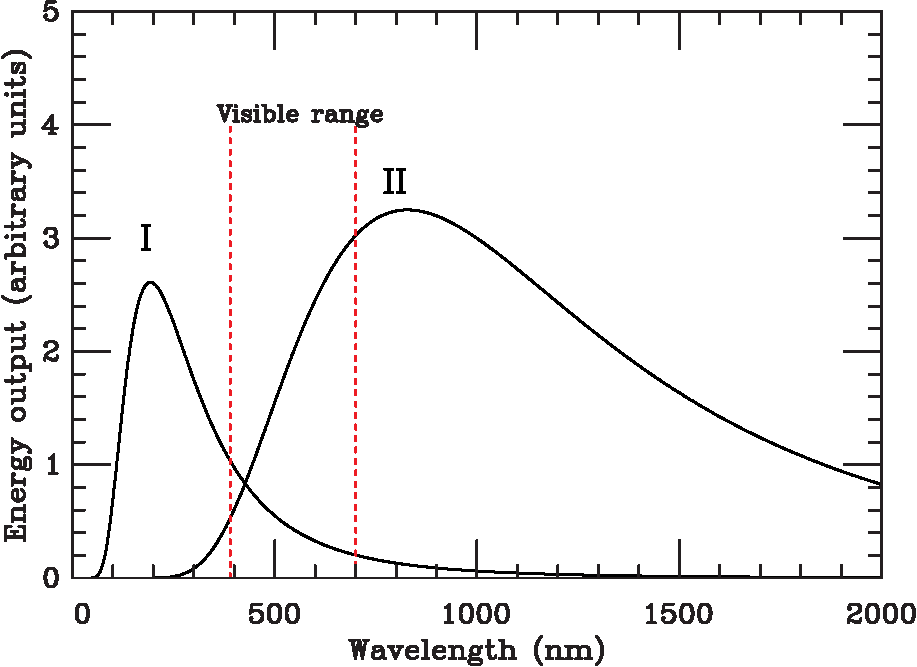
\includegraphics[width=2.5in]{twostars-crop.pdf}
	\end{minipage}

\newpage
\item You observe three objects that produce the spectral curves shown here.

\begin{minipage}{0.5\textwidth}
	
	\begin{enumerate}
		\item What color would each one appear to be glowing {\it to the eye}?
		\item Estimate the temperature of each one based on the light they emit.
		\item Could any of them represent the light emitted by a living human? If so, which one? If not, how do you know?
	\end{enumerate}
\end{minipage}
\hspace{0.05\textwidth}
\begin{minipage}{0.4\textwidth}
	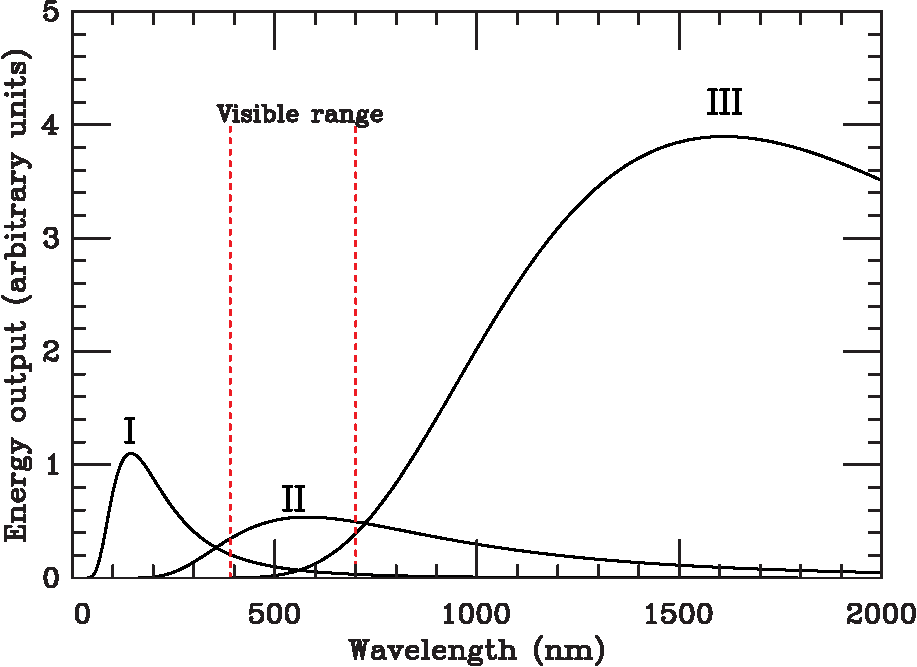
\includegraphics[width=2.5in]{three-objects-crop.pdf}
\end{minipage}


\end{enumerate}




\end{document}


